\clearpage
\item \points{40} {\bf Linear Classifiers (logistic regression and GDA)}

In this problem, we cover two probabilistic linear classifiers we have
covered in class so far. First, a discriminative linear classifier: logistic
regression. Second, a generative linear classifier: Gaussian discriminant
analysis (GDA). Both the algorithms find a linear decision boundary that
separates the data into two classes, but make different assumptions. Our goal
in this problem is to get a deeper understanding of the similarities and
differences (and, strengths and weaknesses) of these two algorithms.

For this problem, we will consider two datasets, provided in the following
files:
\begin{enumerate}[label=\roman*.]
	\item \url{data/ds1_{train,valid}.csv}
	\item \url{data/ds2_{train,valid}.csv}
\end{enumerate}
Each file contains $m$ examples, one example $(x^{(i)}, y^{(i)})$ per row.
In particular, the $i$-th row contains columns $x^{(i)}_0\in\Re$,
$x^{(i)}_1\in\Re$, and $y^{(i)}\in\{0, 1\}$. In the subproblems that follow, we
will investigate using logistic regression and Gaussian discriminant analysis
(GDA) to perform binary classification on these two datasets.

\begin{enumerate}
	\item \subquestionpoints{5}
Show that the above property holds true for the described logistic regression
model over the range $(a,b) = (0,1)$.

\textit{Hint}: Use the fact that we include a bias term.

\ifnum\solutions=1 {
  \begin{answer}
    $$
        \frac{\partial}{\partial \theta_j} \ell(\theta) = \sum_{i=1}^m (y^{(i)} - h_\theta(x^{(i)}))x^{(i)}_j \\
    $$  
    Let $\frac{\partial}{\partial \theta_j} \ell(\theta) = 0$, $j = 0$(thus for any i, $x^{(i)}_j = 1$), then
    $$
    \begin{aligned}
        \sum_{i = 1}^m (y^{(i)} - h_\theta(x^{(i)})) &= 0 \\
        \sum_{i = 1}^m h_\theta(x^{(i)}) &= \sum_{i = 1}^m y^{(i)} \\
    \end{aligned}
    $$ 
    which leads to the result we want to prove.
\end{answer}

} \fi

	\clearpage
\item \subquestionpoints{5} \textbf{Coding problem.}
Follow the instructions in \texttt{src/p01b\_logreg.py} to train a
logistic regression classifier using Newton's Method.
Starting with $\theta = \vec{0}$, run Newton's Method until the updates to
$\theta$ are small: Specifically,  train until the first iteration $k$ such
that $\|\theta_{k} - \theta_{k-1}\|_1 < \epsilon$, where
$\epsilon = 1\times 10^{-5}$. Make sure to write your model's predictions to
the file specified in the code.

\ifnum\solutions=1 {
  \begin{answer}
\end{answer}

} \fi

	\clearpage
\item \subquestionpoints{5}
Recall that in GDA we model the joint distribution of $(x, y)$ by the following
equations:
%
\begin{eqnarray*}
	p(y) &=& \begin{cases}
	\phi & \mbox{if~} y = 1 \\
	1 - \phi & \mbox{if~} y = 0 \end{cases} \\
	p(x | y=0) &=& \frac{1}{(2\pi)^{n/2} |\Sigma|^{1/2}}
		\exp\left(-\frac{1}{2}(x-\mu_{0})^T \Sigma^{-1} (x-\mu_{0})\right) \\
	p(x | y=1) &=& \frac{1}{(2\pi)^{n/2} |\Sigma|^{1/2}}
		\exp\left(-\frac{1}{2}(x-\mu_1)^T \Sigma^{-1} (x-\mu_1) \right),
\end{eqnarray*}
%
where $\phi$, $\mu_0$, $\mu_1$, and $\Sigma$ are the parameters of our model.

Suppose we have already fit $\phi$, $\mu_0$, $\mu_1$, and $\Sigma$, and now
want to predict $y$ given a new point $x$. To show that GDA results in a
classifier that has a linear decision boundary, show the posterior distribution
can be written as
%
\begin{equation*}
	p(y = 1\mid x; \phi, \mu_0, \mu_1, \Sigma)
	= \frac{1}{1 + \exp(-(\theta^T x + \theta_0))},
\end{equation*}
%
where $\theta\in\Re^n$ and $\theta_{0}\in\Re$ are appropriate functions of
$\phi$, $\Sigma$, $\mu_0$, and $\mu_1$.

\ifnum\solutions=1{
  \begin{answer}
    $$
    \begin{aligned}
        p(y=1|x;\phi,\mu_0,\mu_1,\Sigma) &= \frac{p(x|y=1)p(y=1)}{p(x|y=0)p(y=0)+p(x|y=1)p(y=1)} \\
        &= \frac{1}{1+\frac{p(x|y=0)p(y=0)}{p(x|y=1)p(y=1)}} \\
        &= \frac{1}{1+\frac{1-\phi}{\phi}\exp{(\frac{1}{2}(x-\mu_1)^T\Sigma^{-1}(x-\mu_1) - \frac{1}{2}(x-\mu_0)^T\Sigma^{-1}(x-\mu_0)}} \\
        &=\frac{1}{1+\frac{1-\phi}{\phi}\exp{((\mu_0-\mu_1)^T\Sigma^{-1}x+\frac{1}{2}(\mu_1^T\Sigma^{-1}\mu_1 - }\mu_0^T\Sigma^{-1}\mu_0))}\\
        &=\frac{1}{1+\exp{\{-[(\mu_1-\mu_0)^T\Sigma^{-1}x+\frac{1}{2}(\mu_0^T\Sigma^{-1}\mu_0 - }\mu_1^T\Sigma^{-1}\mu_1)+\ln{(\frac{\phi}{1-\phi})}]\}}\\
        &=\frac{1}{1+\exp{(-(\theta^Tx+\theta_0))}}
        \end{aligned}\\
    $$
    note that $\Sigma$ is symmetric, so we have:
    $$
        \begin{aligned}
        \theta &= (\Sigma^{-1})^T(\mu_1-\mu_0) = \Sigma^{-1}(\mu_1-\mu_0)\\ 
        \theta_0 &=\frac{1}{2}(\mu_0^T\Sigma^{-1}\mu_0-\mu_1^T\Sigma^{-1}\mu_1)+\ln{\frac{\phi}{1-\phi}}
        \end{aligned}
    $$

\end{answer}

}\fi

	\clearpage
\item \subquestionpoints{7} For this part of the problem only, you may
  assume $n$ (the dimension of $x$) is 1, so that $\Sigma = [\sigma^2]$ is
  just a real number, and likewise the determinant of $\Sigma$ is given by
  $|\Sigma| = \sigma^2$.  Given the dataset, we claim that the maximum
  likelihood estimates of the parameters are given by
  \begin{eqnarray*}
    \phi &=& \frac{1}{m} \sum_{i=1}^m 1\{y^{(i)} = 1\} \\
\mu_{0} &=& \frac{\sum_{i=1}^m 1\{y^{(i)} = {0}\} x^{(i)}}{\sum_{i=1}^m
1\{y^{(i)} = {0}\}} \\
\mu_1 &=& \frac{\sum_{i=1}^m 1\{y^{(i)} = 1\} x^{(i)}}{\sum_{i=1}^m 1\{y^{(i)}
= 1\}} \\
\Sigma &=& \frac{1}{m} \sum_{i=1}^m (x^{(i)} - \mu_{y^{(i)}}) (x^{(i)} -
\mu_{y^{(i)}})^T
  \end{eqnarray*}
  The log-likelihood of the data is
  \begin{eqnarray*}
\ell(\phi, \mu_{0}, \mu_1, \Sigma) &=& \log \prod_{i=1}^m p(x^{(i)} , y^{(i)};
\phi, \mu_{0}, \mu_1, \Sigma) \\
&=& \log \prod_{i=1}^m p(x^{(i)} | y^{(i)}; \mu_{0}, \mu_1, \Sigma) p(y^{(i)};
\phi).
  \end{eqnarray*}
By maximizing $\ell$ with respect to the four parameters,
prove that the maximum likelihood estimates of $\phi$, $\mu_{0}, \mu_1$, and
$\Sigma$ are indeed as given in the formulas above.  (You may assume that there
is at least one positive and one negative example, so that the denominators in
the definitions of $\mu_{0}$ and $\mu_1$ above are non-zero.)

\ifnum\solutions=1 {
  \begin{answer}
    $$
    \begin{aligned}
        \ell(\phi, \mu_{0}, \mu_1, \Sigma) 
        &= \log \prod_{i=1}^m p(x^{(i)} , y^{(i)};\phi, \mu_{0}, \mu_1, \Sigma) \\
        &= \log \prod_{i=1}^m p(x^{(i)} | y^{(i)}; \mu_{0}, \mu_1, \Sigma) p(y^{(i)};\phi)\\
        &=\sum_{i = 1}^m \log{p(x^{(i)} | y^{(i)}; \mu_{0}, \mu_1, \Sigma)} + \sum_{i = 1}^m \log p(y^{(i)};\phi) \\
        &=-\frac{mn}{2}\log{2\pi}--\frac{m}{2}\log{|\Sigma|}-
        \frac{1}{2}\sum_{i=1}^m(x^{(i)}-\mu_{y^{(i)}})^T\Sigma^{-1}(x^{(i)}-\mu_{y^{(i)}})\\
        &+\sum_{i=1}^m \left(y^{(i)}\log{\phi}+(1-y^{(i)})\log{(1-\phi)}\right)
    \end{aligned}\\
    $$

    $$
    \begin{aligned}
        \frac{\partial\ell}{\partial \phi} &=0+\left(\frac{\sum_{i = 1}^m 1\{y^{(i)}=1\}}{\phi}-\frac{\sum_{i = 1}^m 1\{y^{(i)}=0\}}{1-\phi}\right)\\
        &=\frac{\sum_{i = 1}^m 1\{y^{(i)}=1\}-\sum_{i = 1}^m 1\{y^{(i)}=1\}\phi-\sum_{i = 1}^m 1\{y^{(i)}=0\}\phi}{\phi(1-\phi)} \\
        &=\frac{\sum_{i = 1}^m 1\{y^{(i)}=1\}-m\phi}{\phi(1-\phi)}\\
        \ \\
        \frac{\partial\ell}{\partial \mu_0} &= \frac{\partial\ell}{\partial \mu_{y^{(i)}}}\frac{\partial\mu_{y^{(i)}}}{\partial \mu_0} \\
        &=\sum_{i = 1}^m\frac{x^{(i)}-\mu_{y^{(i)}}}{|\Sigma|}1\{y^{(i)}=0\}\\
        &=\frac{\sum_{i = 1}^m1\{y^{(i)}=0\}x^{(i)}-\sum_{i = 1}^m1\{y^{(i)}=0\}\mu_0}{|\Sigma|}\\
        \ \\
        \frac{\partial\ell}{\partial \mu_1} &=\frac{\sum_{i = 1}^m1\{y^{(i)}=1\}x^{(i)}-\sum_{i = 1}^m1\{y^{(i)}=1\}\mu_1}{|\Sigma|}\\
        \ \\
        \frac{\partial \ell}{\partial\Sigma} &= \frac{\partial}{\partial \Sigma}\left(\sum_{i = 1}^m(-\frac{1}{2}\log{\Sigma-\frac{(x^{(i)}-\mu_{y^{(i)}})^T(x^{(i)}-\mu_{y^{(i)}})}{2\Sigma}}) \right) \\
        &=-\frac{1}{2}\left(\frac{m}{\Sigma}-\frac{\sum_{i = 1}^m(x^{(i)}-\mu_{y^{(i)}})^T(x^{(i)}-\mu_{y^{(i)}})}{\Sigma^2} \right) \\
        &=-\frac{m\Sigma-\sum_{i = 1}^m(x^{(i)}-\mu_{y^{(i)}})^T(x^{(i)}-\mu_{y^{(i)}})}{2\Sigma^2}\\
    \end{aligned}  \\
    $$
    
    $$
    \begin{aligned}
        \frac{\partial\ell}{\partial \phi} &= 0\\
        \frac{\partial\ell}{\partial \mu_0} &= 0\\
        \frac{\partial\ell}{\partial \mu_1} &= 0\\
        \frac{\partial\ell}{\partial \Sigma} &= 0\\
    \end{aligned}
    \Rightarrow 
    \begin{aligned}
        \phi &= \frac{1}{m} \sum_{i=1}^m 1\{y^{(i)} = 1\} \\
        \mu_{0} &= \frac{\sum_{i=1}^m 1\{y^{(i)} = {0}\} x^{(i)}}{\sum_{i=1}^m
            1\{y^{(i)} = {0}\}} \\
        \mu_1 &= \frac{\sum_{i=1}^m 1\{y^{(i)} = 1\} x^{(i)}}{\sum_{i=1}^m 1\{y^{(i)}
        = 1\}} \\
        \Sigma &= \frac{1}{m} \sum_{i=1}^m (x^{(i)} - \mu_{y^{(i)}}) (x^{(i)} -
        \mu_{y^{(i)}})^T
    \end{aligned}
    $$
\end{answer}

} \fi

	\clearpage
\item \subquestionpoints{3} \textbf{Coding problem.}
In \texttt{src/p01e\_gda.py}, fill in the code to
calculate $\phi$, $\mu_{0}$, $\mu_{1}$, and $\Sigma$, use these parameters
to derive $\theta$, and use the resulting GDA model to make predictions on the
validation set.

\ifnum\solutions=1 {
  \begin{answer}
\end{answer}

} \fi

	\clearpage
\item \subquestionpoints{5}
For Dataset 1, create a plot of the validation set with $x_1$ on the horizontal
axis, and $x_2$ on the vertical axis. To visualize the two classes, use a
different symbol for examples $x^{(i)}$ with $y^{(i)} = 0$ than for those with
$y^{(i)} = 1$. On the same figure, plot the decision boundary found by logistic
regression in part (b). Make an identical plot with the decision boundary found
by GDA in part (e).

\ifnum\solutions=1 {
\begin{answer}
    \begin{figure}[htbp]
        \centering
        \begin{minipage}[t]{0.48\textwidth}
        \centering
        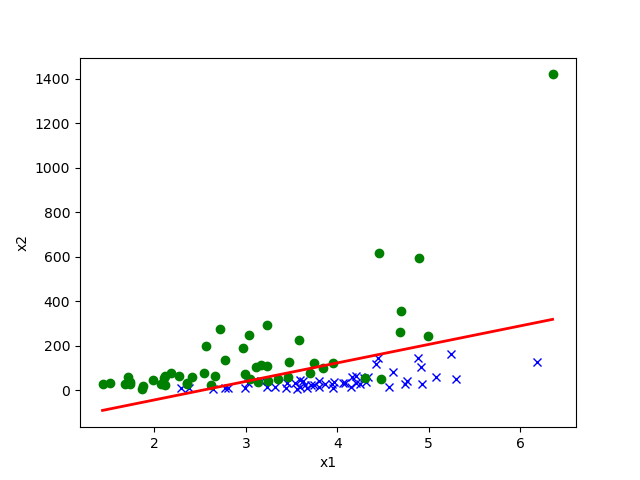
\includegraphics[width=6cm]{../src/output/p01b_pred_1.png}
        \caption{Logistic Regression on Dataset 1}
        \end{minipage}
        \begin{minipage}[t]{0.48\textwidth}
        \centering
        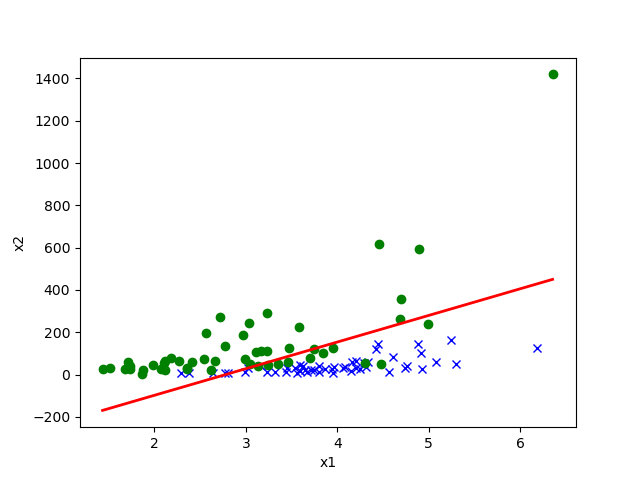
\includegraphics[width=6cm]{../src/output/p01e_pred_1.png}
        \caption{GDA on Dataset 1}
        \end{minipage}
    \end{figure}
\end{answer}

} \fi

	\clearpage
\item \subquestionpoints{5}
Repeat the steps in part (f) for Dataset 2. On which dataset does GDA seem to
perform worse than logistic regression? Why might this be the case?

\ifnum\solutions=1{
  \begin{answer}
    \begin{figure}[htbp]
        \centering
        \begin{minipage}[t]{0.48\textwidth}
        \centering
        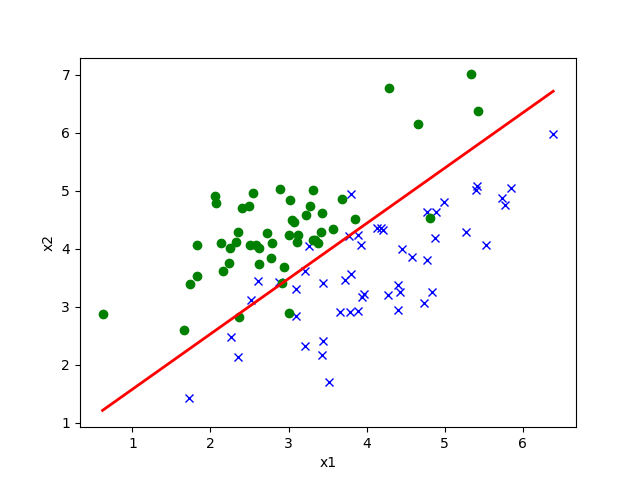
\includegraphics[width=6cm]{../src/output/p01b_pred_2.png}
        \caption{Logistic Regression on Dataset 2}
        \end{minipage}
        \begin{minipage}[t]{0.48\textwidth}
        \centering
        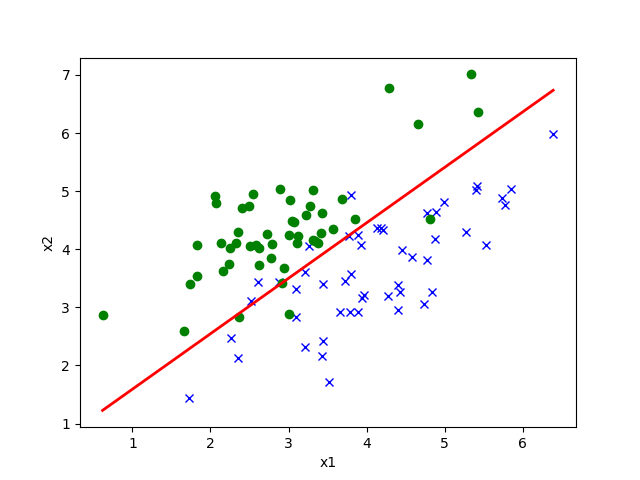
\includegraphics[width=6cm]{../src/output/p01e_pred_2.png}
        \caption{GDA on Dataset 2}
        \end{minipage}
    \end{figure}

    On dataset 1 GDA perform worse than logistic regression, since the distribution of dataset 1 is non-Gaussian. Logistic regression makes 
    weaker assumptions, and is more robust to deviations from modeling assumptions.
\end{answer}

}\fi

	\clearpage
\item \points{3 extra credit} For the dataset where GDA performed worse in
parts (f) and (g), can you find a transformation of the $x^{(i)}$'s such
that GDA performs significantly better? What is this transformation?

\ifnum\solutions=1{
  \begin{answer}
    
    To be continued.
\end{answer}

}\fi

\end{enumerate}
